% !TEX root = ../ClassicThesis_DEIB.tex

\chapter{Grape hardware and software Architecure} \label{chap:grapeSoftwareArchitecture}

In this chapter we are going to describe in a detailed way the architecture of the robotic platform we used to implement the system to fulfill the requirements described in Section \ref{sec:grapeProjectDescription}. First, in Section \ref{sec:grapeHwArch}, we are giving an overview of the hardware components, from the robot base to all the actuators/sensors present on board. In Section \ref{sec:grapeSwArch}, we'll start to analyze the software architecure of the system, explaining what the main modules are, and the relationships between them.

\section{GRAPE hardware architecture}\label{sec:grapeHwArch}

\subsection{Robotic Base}
The choice of the robotic base is, of course, a crucial point in the development of our system, for two reasons:
\begin{itemize}
	\item without a well-functioning robotic base, no other objective can be achieved
	\item the vineyard environment is particularly challenging in nature (this particular aspect will be well-justified in Chapter \ref{chap:localization}), so we cannot rely on a non-prudent choice.
\end{itemize}
As anticipated in Section \ref{sec:odometry}, the choice fell on the \textbf{Husky} \ac{UGV} from Clearpath Robotics\footnote{\url{https://www.clearpathrobotics.com/husky-unmanned-ground-vehicle-robot/}},
(see Figure \ref{fig:husky}). There are several reasons for the adoption of this specific model:
\begin{itemize}
	\item it's a widely used platform (\textit{e.g.}: \cite{husky1}; \cite{husky2}; \cite{husky3})
	\item it has a \textit{skid steering} kinematics that, as already seen in Section \ref{sec:odometry}, can be essentially reduced to a \textit{differential drive} kinematics, that is very simple.
	\item it's specifically designed for outdoor use, so robustness and ability to deal with unstructured terrain are problems addressed by its rugged construction and high-torque drivetrain.
	\item it offers a large payload capacity, to host the moltitude of sensors, actuators and computational units we need
	\item it's fully supported in \ac{ROS}, with open source drivers, configuration files and examples
\end{itemize}

\begin{figure}
	\centering
	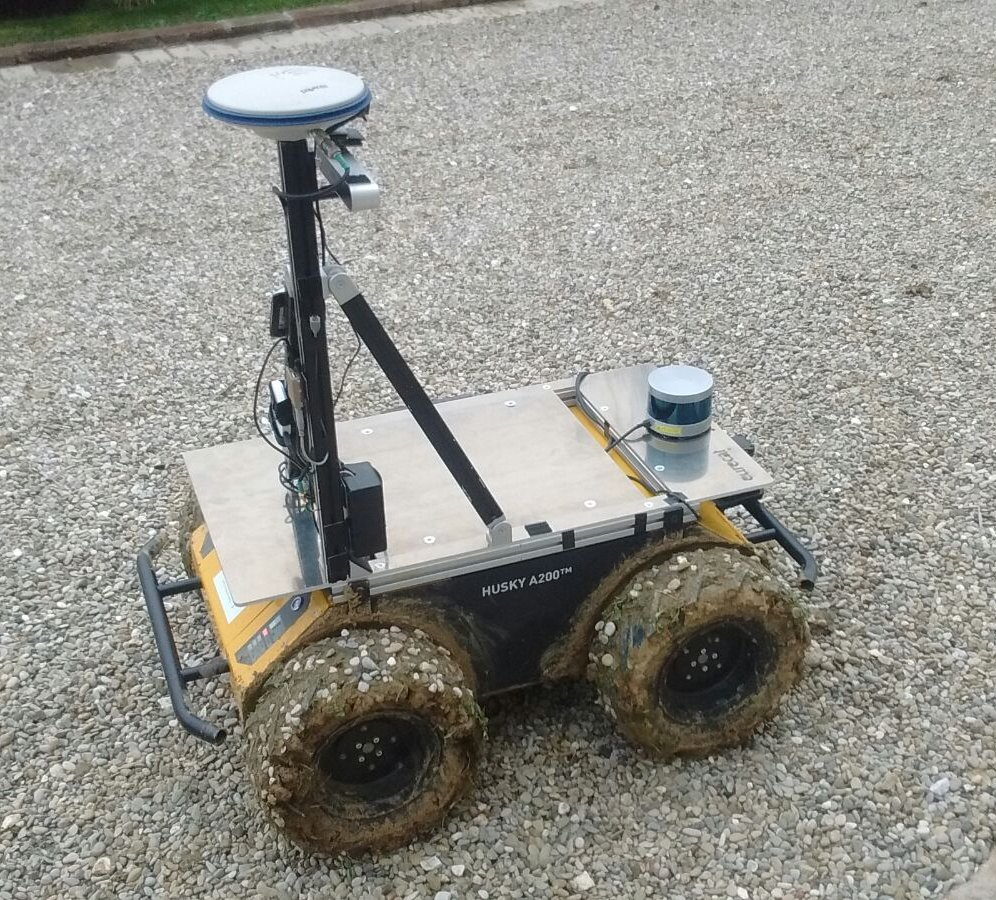
\includegraphics[width=0.5\textwidth]{Images/grape_sw_hw_architecture/ruoteFangose.jpeg}
	\caption{\textit{Husky platform after a navigation session in environment. You can easily note the amount of stones and mud stuck into the wheels.}}
	\label{fig:ruoteFangose}
\end{figure}

This choice turned out to be substantially good. The wheels odometry turned out to be  better than expected (TODO grafico della posizione xy dell'odometry delle ruote vs grafico della posizione stimata con robot localization), and the \ac{ROS} drivers and config files were actually pretty easy to use and modify. The only major weakness identified in the Husky is related to its behavior on muddy ground, and is due to the wheels shape. In effect, after a few minutes of navigation in the mud, the \ac{UGV} tends to collect a significative amount of earth and stones in the wheels groves (see Figure \ref{fig:ruoteFangose}) and, consequentely, lose grip on the ground. This problem is likely to be attenuated or solved by use of tracks instead of wheels.

\subsection{Robotic Arm}\label{subsec:kinovaArm}
By observing how pherormone dispensers must be deployed on the vine plant in Figure \ref{fig:dispensers} (in Figure \ref{fig:dispenserNostro}, you can see the dispenser shape that we actually used for \ac{GRAPE} project), it's easy to understand that we require a very flexible robotic arm, with advanced capacity of movement and capable of precise movement. Additional constraints also come from the limited space available on the Husky base, and from the limited power supply at disposal aboard. The choice fell on \textit{Jaco$^2$} arm from Kinova Robotics\footnote{\url{http://www.kinovarobotics.com/wp-content/uploads/2017/06/JACO\%C2\%B2-User-Guide-Asstive-Robotics-April-2017.pdf}}
(see Figure \ref{fig:kinovaArm}, Table \ref{tab:kinovaArmSpecs} for product specifications), for these reasons:
\begin{itemize}
	\item 6 DOF provide the required flexibility
	\item 3 fingers can be used for the dispensers deployment
	\item while programmatic control is necessary for \ac{GRAPE} purpose, the joystick control make it easy to perform quick tests and analyze the robot capabilities
	\item unlimited joints rotations
	\item reduced weight and power consumption
	\item small overall dimensions
	\item \ac{ROS} open source drivers already provided by Kinova Robotics
\end{itemize}


\begin{table}[tb]
\footnotesize
\centering
\begin{tabularx}{0.6\textwidth}{lr}
\toprule
\tableheadline{l}{Parameter}  &
\tableheadline{r}{Value}  \\
\midrule
\tablefirstcol{l}{Degrees of Freedom}
& 6 \\
\midrule
\tablefirstcol{l}{Weight}
& 5.2 Kg \\
\midrule
\tablefirstcol{l}{Payload}
& 1.3 Kg \\
\midrule
\tablefirstcol{l}{Reach}
& 90 cm \\
\midrule
\tablefirstcol{l}{Maximum Linear arm speed}
& 20 $cm/s$ \\
\midrule
\tablefirstcol{l}{Power supply}
& $18\div29$ VDC \\
\midrule
\tablefirstcol{l}{Average Power}
& 25W \\
\midrule
\tablefirstcol{l}{Peak power}
& 100W \\
\midrule
\tablefirstcol{l}{Communication Protocol}
& RS485 \\
\midrule\tablefirstcol{l}{Material}
& Carbon fiber \\
\bottomrule
\end{tabularx}
\caption[Kinova Jaco$^2$ product specification]{Product specifications of Jaco$^2$ from Kinova Robotics.}
\label{tab:kinovaArmSpecs}
\end{table}


\begin{figure}
	\centering
	\subfloat[]{%
		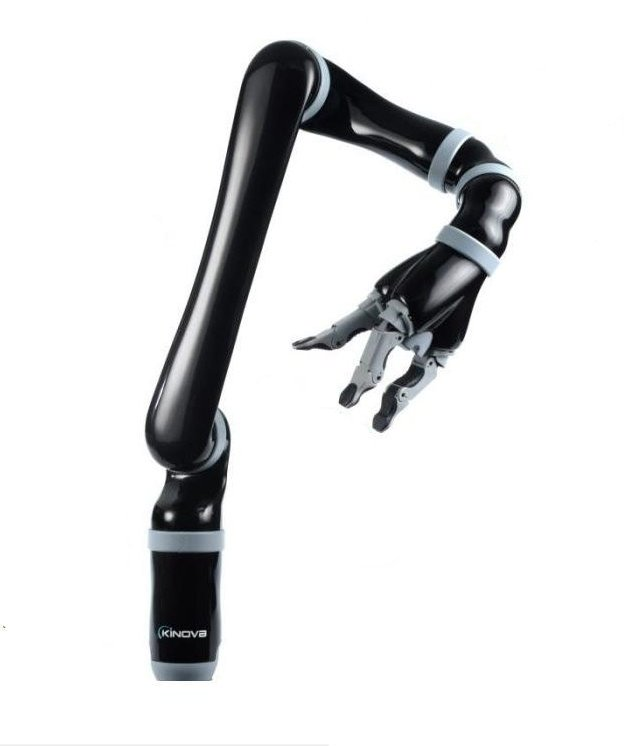
\includegraphics[width=0.45\textwidth]{Images/grape_sw_hw_architecture/kinova.jpg}
		\label{fig:kinovaArm}}
	\qquad
	\subfloat[]{%
		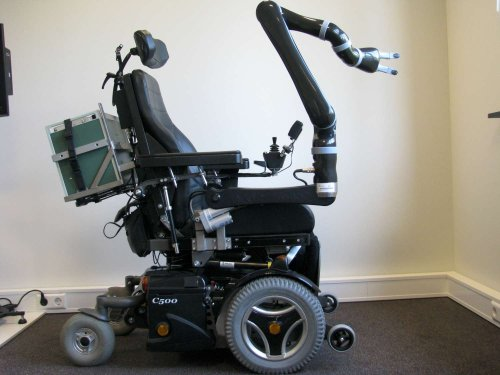
\includegraphics[width=0.4\textwidth]{Images/grape_sw_hw_architecture/kinovaCarrozzina.jpg}
		\label{fig:kinovaCarrozzina}}
	\caption{\textit{Robotic arm Jaco$^2$ with 3 fingers, from Kinova Robotics (\ref{fig:kinovaArm}) and the same arm mounted on a wheelchair \ref{fig:kinovaCarrozzina}}}
\end{figure}

 Some of the nice features of this device (weight, dimensions) actually derive from the original purpose of the arm, that is placed in the context of assistive devices for disabled people, to improve quality of life and independence of people on  power wheelchairs (see Figure \ref{fig:kinovaCarrozzina}). But this fact also brought some unexpected weaknesses, that introduced a series quite serious problems that slowed down the development process. The identified weaknesses are:
 \begin{itemize}
 	\item a very large imprecision in the movements piloted via programmatic control: this is probably due to joystick control seen as a "main mode" control since, as previously stated, the arm is born as an assistive device. This problem was partially solved modifying the open source drivers of the arm, but entire control strategies were introduced to compensate this weakness.
 	\item buggy implementation of joints constraints, probably due to the same cause of the previous point. This created a major problem mostly because of the wiring used for the sensors (described in next Sections) mounted on the arm, that kept rolling up because of the unlimited joints rotations. TODO a seconda di come alla fine la risolviamo definitivamente (messi a posto i driver, o procedure di controllo) lo scrivo.
 \end{itemize}
 
After the analysis of the macro goals of \ac{GRAPE} project (Section \ref{sec:grapeProjectDescription}), it was decided to use the arm as a support for other sensors, as well as manipulation tool, for the dispenser deployment task: a \ac{LIDAR} and an RGB-D camera (see Image \ref{} TODO fai foto a come i sensori sono montati sull'end effector).
 
 \subsection{LIDARs}
 
 The final robotic system mounts three different \ac{LIDAR}s: two in front of the Husky for visualization and navigation purposes, and the other one mounted on a metal support on top of the arm end effector. The purpose of this last \ac{LIDAR} will be cleared in Chapter \ref{chap:kinovaArmChapter}; for now, all you need to know is that it's used in the procedure of identification of the most suitable point for dispenser deployment. The \ac{LIDAR}s come from different producers, but they are quite similar being designed for outdoor use. The two used for navigation are \textbf{Velodyne VLP-16}\footnote{\url{http://velodynelidar.com/vlp-16-lite.html}}
 and \textbf{Hokuyo UTM-30LX-EW}\footnote{\url{https://www.hokuyo-aut.jp/search/single.php?serial=170}},
 the one on top of the arm is \textbf{SICK Tim561}\footnote{\url{https://www.sick.com/de/en/detection-and-ranging-solutions/2d-lidar-sensors/tim5xx/tim561-2050101/p/p369446}}.
 Main differences and similarities between these models are highlighted in Table \ref{tab:lidarComparison}


\begin{table}[tb]
\footnotesize
\centering
\begin{tabularx}{0.85\textwidth}{llll}
\toprule
\tableheadline{l}{}  &
\tableheadline{r}{VLP-16}  &
\tableheadline{r}{Tim561}  &
\tableheadline{r}{UTM-30LX-EW}  \\
\midrule
\tablefirstcol{l}{Number of Channels}
&16  &1 & 1\\
\midrule
\tablefirstcol{l}{Scan Angle}
&360°  & 270° & 270°\\
\midrule
\tablefirstcol{l}{Rotation rate}
&5Hz    & 15 Hz & 40Hz \\
&10Hz &  & \\
&20Hz &   & \\
\midrule
\tablefirstcol{l}{Angular Resolution}
& 0.1° & 0.33° & 025° \\
& 0.2°&\\
& 0.4°&\\
\midrule
\tablefirstcol{l}{Range}
&100m  & 10m & 30m\\
\midrule
\tablefirstcol{l}{Power Consumption}
&8W  & 4W& <8W\\
\midrule
\tablefirstcol{l}{Weight}
&590g  & 250g & 210g\\
\bottomrule
\end{tabularx}
\caption[\ac{LIDAR}s comparison]{Comparison of onboard \ac{LIDAR}s }
\label{tab:lidarComparison}
\end{table}


\begin{figure}
	\centering
	\subfloat[]{%
		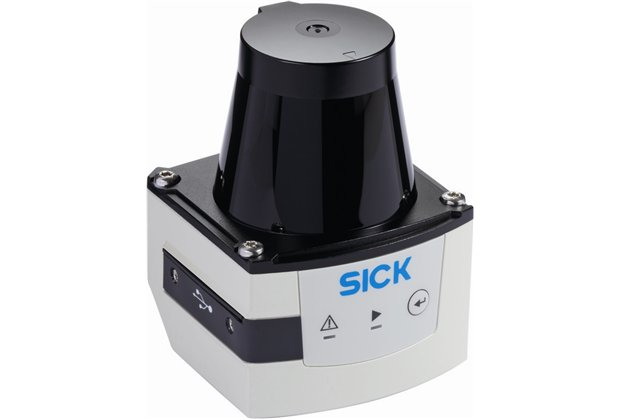
\includegraphics[width=0.35\textwidth]{Images/grape_sw_hw_architecture/sickTim561.jpg}
		\label{fig:sickTim561}}
%	\qquad
	\subfloat[]{%
		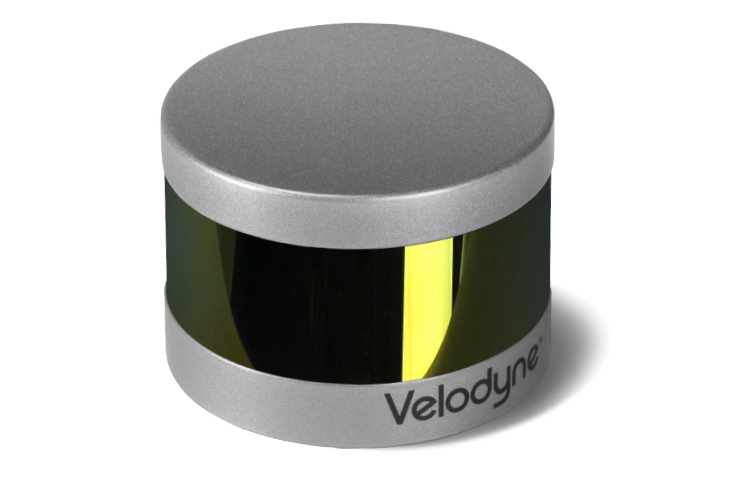
\includegraphics[width=0.3\textwidth]{Images/grape_sw_hw_architecture/velodynePuck.png}
		\label{fig:velodynePuckLite}}
	\subfloat[]{%
		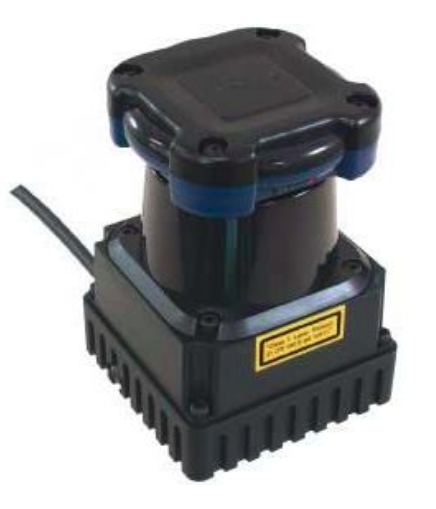
\includegraphics[width=0.25\textwidth]{Images/grape_sw_hw_architecture/hokuyo.png}
		\label{fig:hokuyo}}
	\caption{\textit{Three \ac{LIDAR}s mounted on our \ac{UGV}: Tim561 (\ref{fig:sickTim561}) from SICK, Puck Lite (\ref{fig:velodynePuckLite}) from Velodyne, UTM-30LX-EW \ref{fig:hokuyo} from Hokuyo.}}
\end{figure}

\subsection{RGB-D camera}
The other sensor mounted on top of the arm end effector is an \textbf{RealSense} RGB-D camera from Intel. This camera is able to sense the depth of the acquired images (see Figure TODO screenshot di rgb e profondità), by means of an active infrared stereo technology. The main usage of the camera is to provide images used for the feedback loop of the visual servo control of the Jaco$^2$ arm. Visual servoing is a technique which uses feedback information extracted from a vision sensor to control the motion of a robot \parencite{visualServo}, and it's used in this project to compensate the lack of precision in the arm motion operations (see Section \ref{subsec:kinovaArm}). This camera also applies to operation validation operations (validation of dispenser grasping, validation of dispenser deployment on the plant) and identify exceptional cases (no dispenser left). The positive aspect of this camera model comes from its contained size and weight. We spotted only one significative weak point, that is a quite high minimum depth distance (20 cm), due to the embedded depth technology. This problem created a few complications in dispenser application tasks, but they were easily bypassed.

\subsection{Other sensors}
The \ac{UGV} holds onboard a collection of other sensors, useful for the accomplishment of the established tasks. In this section we'll give a short overview of the few remaining ones:
\begin{description}
	\item[{IMU} sensor] Device including a magnetometer, accelerometer, gyroscope. These sensors were used in the odometry estimation system through sensor fusion algorithms (see Chapter \ref{chap:localization})
	\item[GPS] Also this sensor data stream was included in the odometry estimation system
	\item [Cameras] Additional camera mounted in a slightly lifted position, useful in case of teleoperation of the Husky or the robotic arm and for visualization and monitoring purposes.
\end{description}

 
\section{GRAPE sw architecture}\label{sec:grapeSwArch}


\begin{itemize}
\item Hardware del robot:
		\begin{itemize}
			\item scelta dell'husky (adatto per rugged terrain, supporto di pacchetti ROS), foto
			\item scelta del braccio, con pro (compatto, 6 dof, power consumption non elevata) e contro (movimenti non precisi, fragile, scarso controllo di collisione)
			\item lidar sul braccio per scan
			\item lidar davanti per navigazione e eventualmente localizzazione
			\item camera montata sul braccio
			\item velodyne davanti (a cosa serve?)
			\item camera fissa per eventualmente scattare foto alla vigna
			\item imu
		\end{itemize}
	\item foto del robot 
	%(http://www.grape-project.eu/wp-content/uploads/2017/11/20171030-MacchineTrattori.pdf e eventuali altre che faremo)

\item Software del robot
	\begin{itemize}
		\item descrizione più precisa di quale è nel complesso la procedura: viene dato a mano (interfaccia grafica di Eurecat) una posizione finale, e serie di waypoints intermedi. Procedura di scan che usando PCL trova punti adatti al deployment. Procedura di deploymnet. Waypoint successivo.
		\item struttura col coordinatore, che chiama le 3 action (move\_base, scan, deploy)
		\item di ogni azione, il file che descrive i tipi di goal/result/feedback, con spiegazioni del significato dei parametri
	\end{itemize}
\end{itemize}